\begin{figure}[ht]
\begin{center}
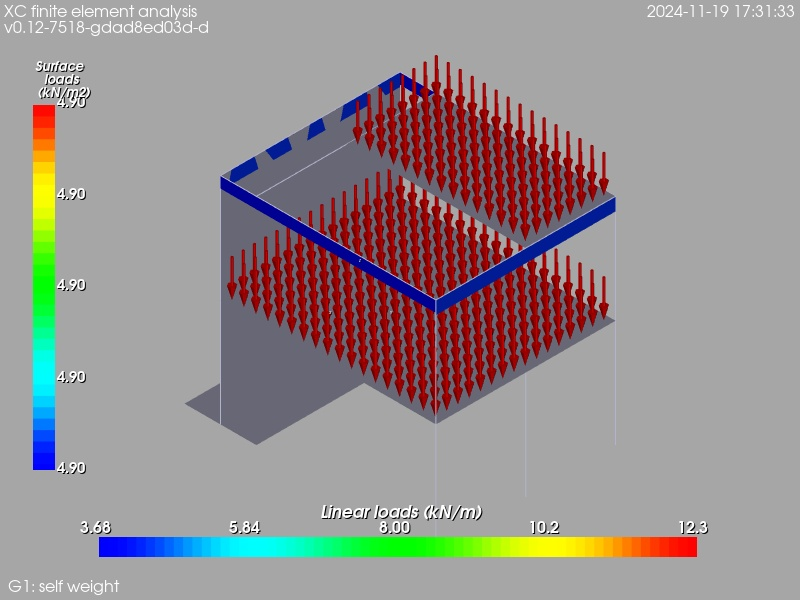
\includegraphics[width=\linewidth]{results/graphics/loads/GselfWeightoverallSet}
\caption{ G1: self weight, distribución de cargas.}
\label{GselfWeightoverallSet}
\end{center}
\end{figure}
\begin{figure}[ht]
\begin{center}
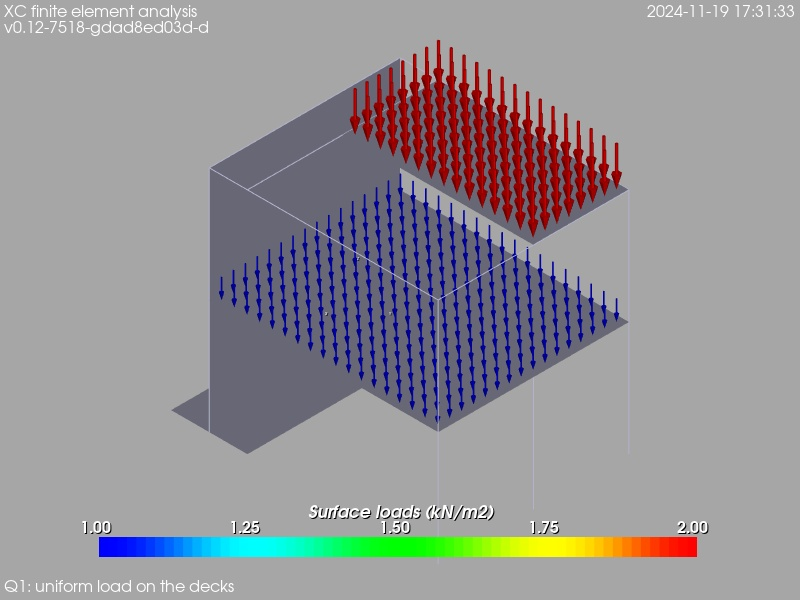
\includegraphics[width=\linewidth]{results/graphics/loads/QdecksoverallSet}
\caption{Q1: uniform load on the decks, distribución de cargas.}
\label{QdecksoverallSet}
\end{center}
\end{figure}
\begin{figure}[ht]
\begin{center}
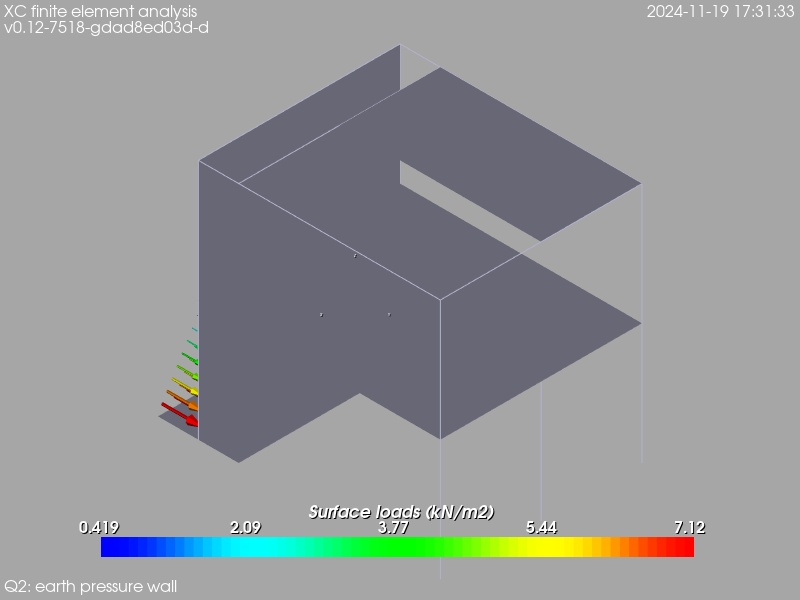
\includegraphics[width=\linewidth]{results/graphics/loads/QearthPressWalloverallSet}
\caption{Q2: earth pressure wall, distribución de cargas.}
\label{QearthPressWalloverallSet}
\end{center}
\end{figure}
\begin{figure}[ht]
\begin{center}
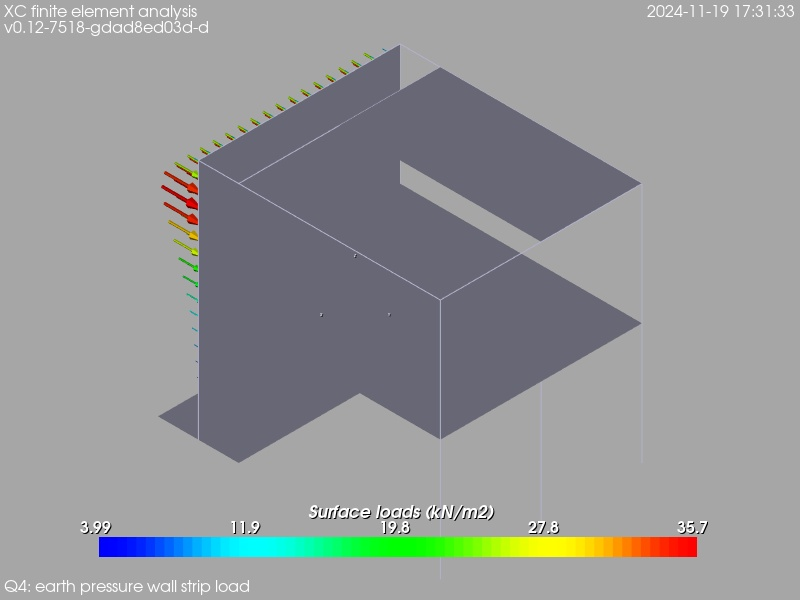
\includegraphics[width=\linewidth]{results/graphics/loads/QearthPWallStrLoverallSet}
\caption{Q4: earth pressure wall strip load, distribución de cargas.}
\label{QearthPWallStrLoverallSet}
\end{center}
\end{figure}
\begin{figure}[ht]
\begin{center}
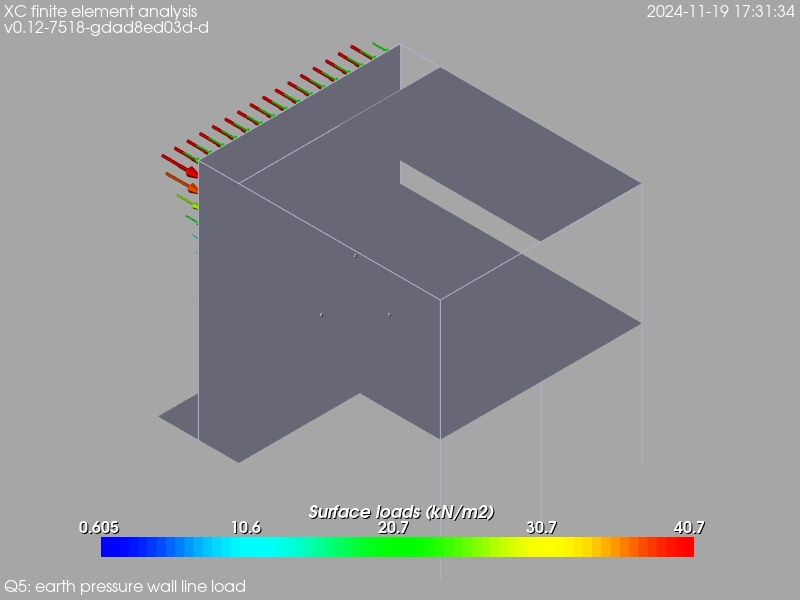
\includegraphics[width=\linewidth]{results/graphics/loads/QearthPWallLinLoverallSet}
\caption{Q5: earth pressure wall line load, distribución de cargas.}
\label{QearthPWallLinLoverallSet}
\end{center}
\end{figure}
\begin{figure}[ht]
\begin{center}
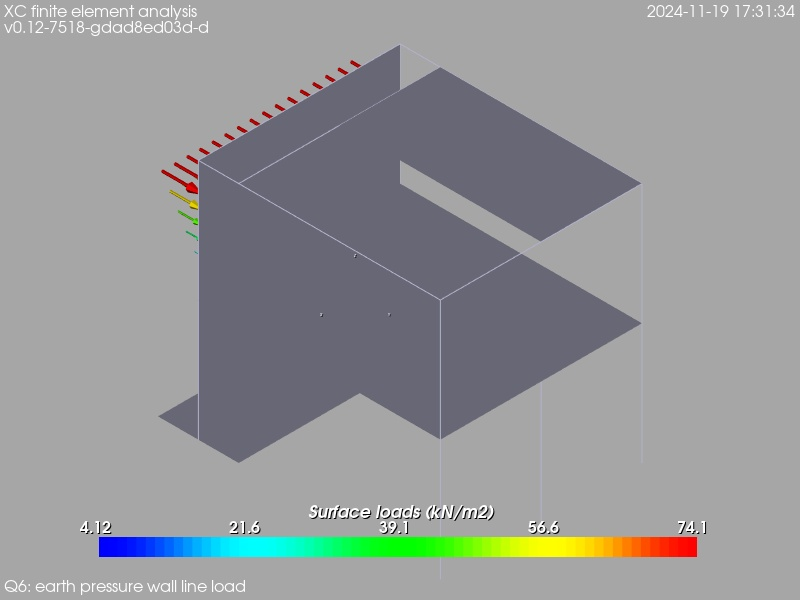
\includegraphics[width=\linewidth]{results/graphics/loads/QearthPWallHrzLoverallSet}
\caption{Q6: earth pressure wall line load, distribución de cargas.}
\label{QearthPWallHrzLoverallSet}
\end{center}
\end{figure}
\begin{figure}[ht]
\begin{center}
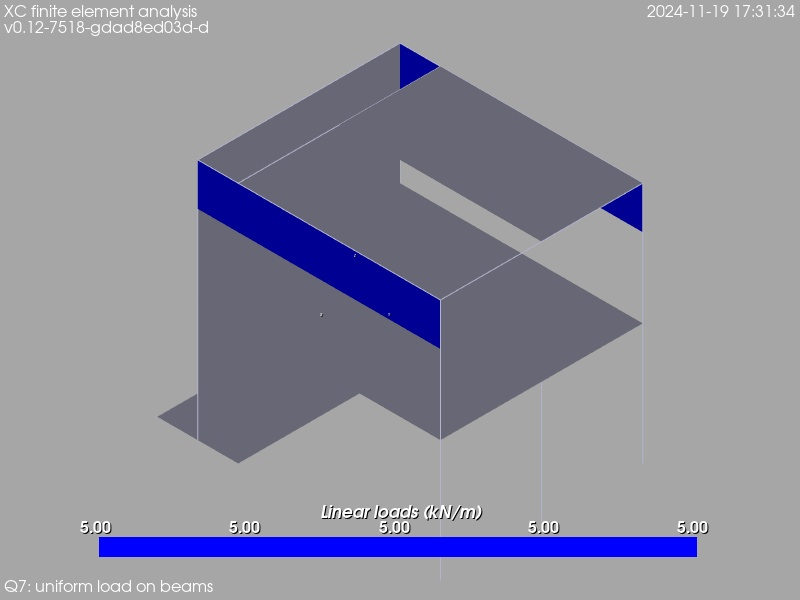
\includegraphics[width=\linewidth]{results/graphics/loads/qunifBeamsoverallSet}
\caption{Q7: uniform load on beams, distribución de cargas.}
\label{qunifBeamsoverallSet}
\end{center}
\end{figure}
\begin{figure}[ht]
\begin{center}
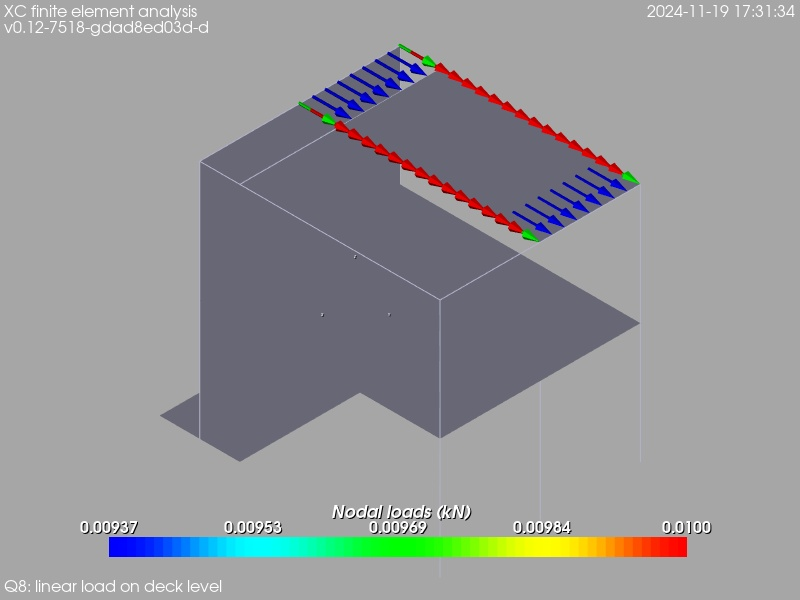
\includegraphics[width=\linewidth]{results/graphics/loads/qlinDeckoverallSet}
\caption{Q8: linear load on deck level , distribución de cargas.}
\label{qlinDeckoverallSet}
\end{center}
\end{figure}
\begin{figure}[ht]
\begin{center}
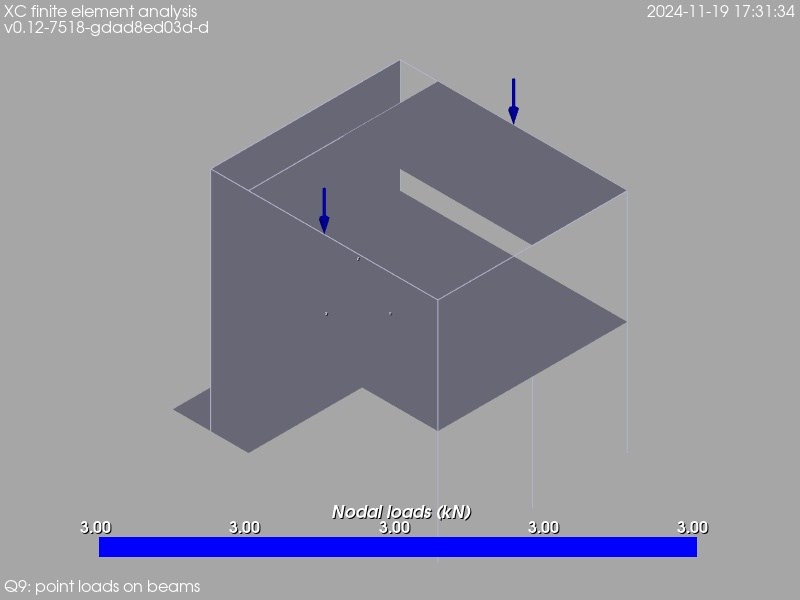
\includegraphics[width=\linewidth]{results/graphics/loads/QpntBeamsoverallSet}
\caption{Q9: point loads on beams, distribución de cargas.}
\label{QpntBeamsoverallSet}
\end{center}
\end{figure}
\begin{figure}[ht]
\begin{center}
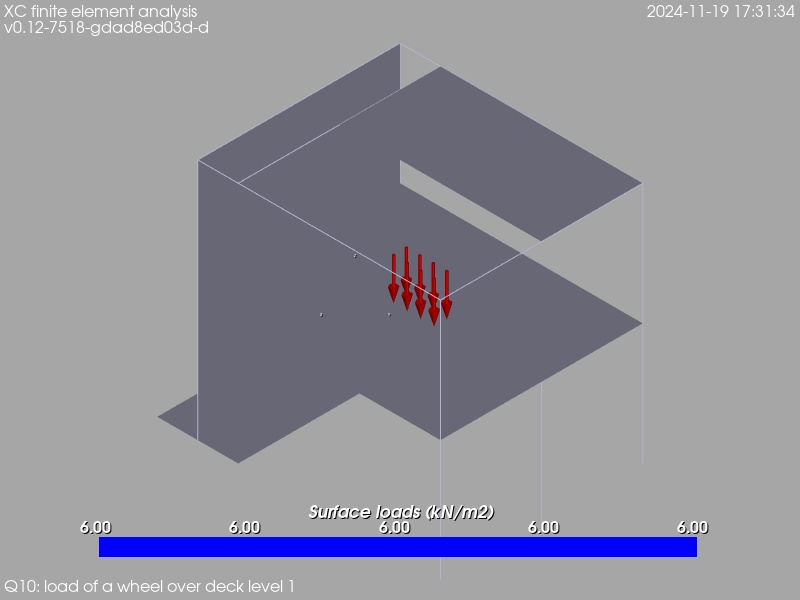
\includegraphics[width=\linewidth]{results/graphics/loads/QwheelDeck1overallSet}
\caption{Q10: load of a wheel over deck level 1, distribución de cargas.}
\label{QwheelDeck1overallSet}
\end{center}
\end{figure}
\begin{figure}[ht]
\begin{center}
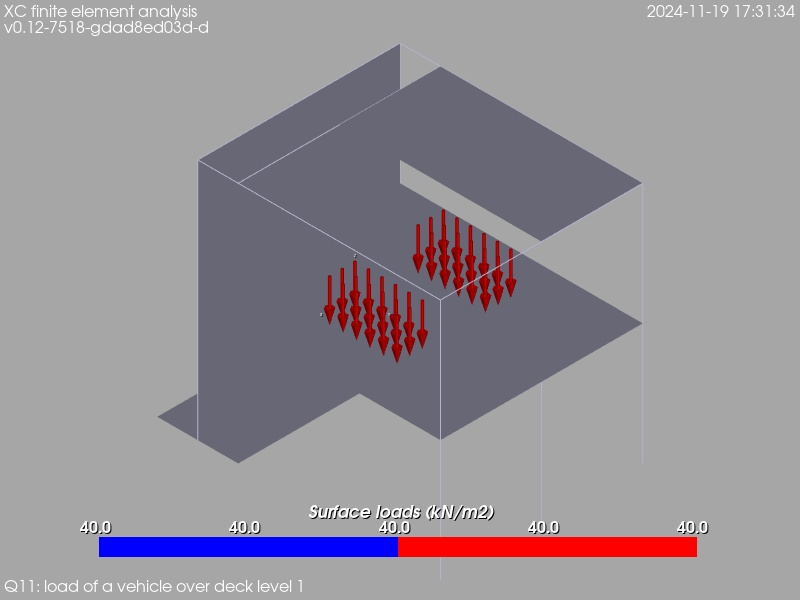
\includegraphics[width=\linewidth]{results/graphics/loads/QvehicleDeck1overallSet}
\caption{Q11: load of a vehicle over deck level 1, distribución de cargas.}
\label{QvehicleDeck1overallSet}
\end{center}
\end{figure}
\begin{figure}[ht]
\begin{center}
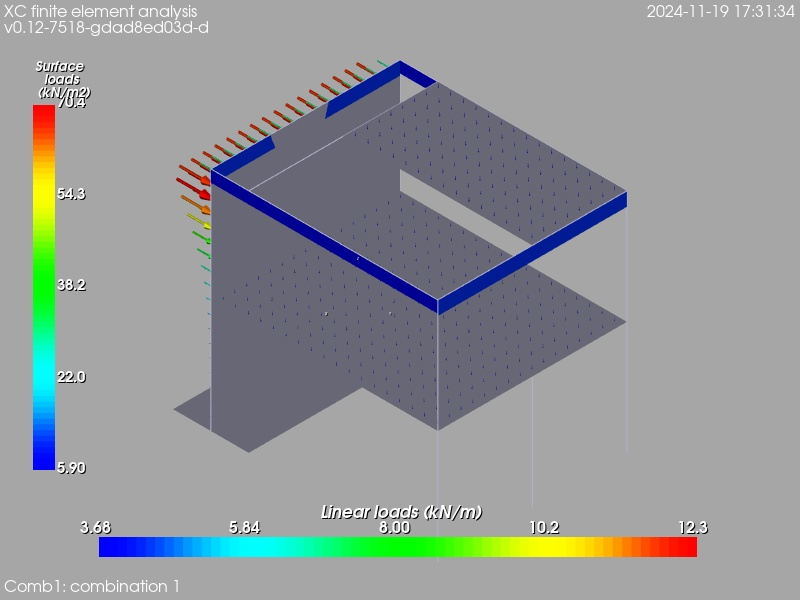
\includegraphics[width=\linewidth]{results/graphics/loads/LS1overallSet}
\caption{Comb1: combination 1, distribución de cargas.}
\label{LS1overallSet}
\end{center}
\end{figure}
\begin{figure}[ht]
\begin{center}
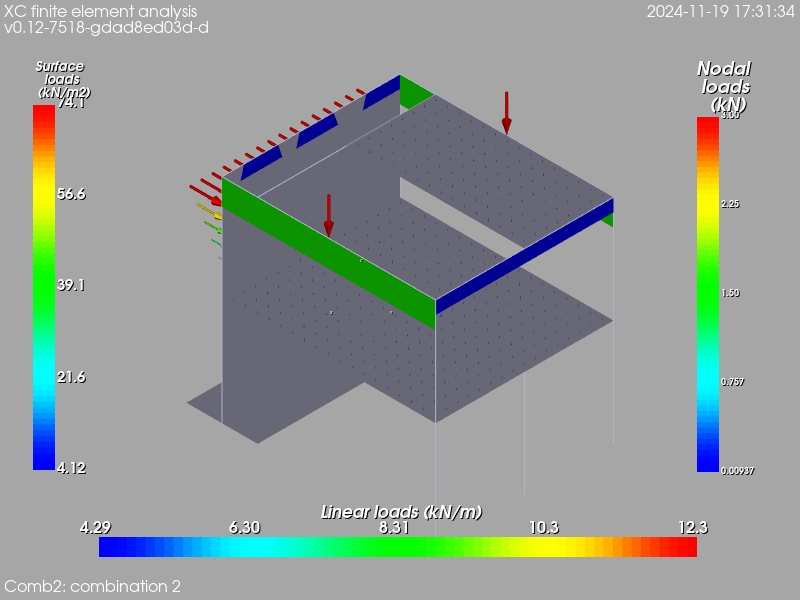
\includegraphics[width=\linewidth]{results/graphics/loads/LS2overallSet}
\caption{Comb2: combination 2, distribución de cargas.}
\label{LS2overallSet}
\end{center}
\end{figure}
